\documentclass[14pt]{extarticle}
\usepackage[spanish]{babel} 
\usepackage[utf8]{inputenc} %Este es el paquete para que te muestre bien los caracteres latinos
\usepackage[useregional]{datetime2} %paquete para la fecha
\usepackage[a4paper]{geometry} %paquete para el tamaño de hoja
\usepackage{changepage} %paquete para cambiar los márgenes a una sola parte del documento con \begin{adjustwidth} y \end{adjustwidth}
\usepackage{lmodern}
%\usepackage{palatino}
\usepackage{fancyhdr} %para los estilos de hoja, también para los l-rhead, l-rfoot
\usepackage{subcaption}
\usepackage[breaklinks=true]{hyperref} %separa las referencias muy largas en varias lineas
\usepackage[pdftex]{graphicx} %paquete para las imágenes
\usepackage[numbers]{natbib}
\graphicspath{ {images/} }
%\usepackage[final]{pdfpages}
%paquete para incorporar pdfs




\newcommand{\fecha}{\today}
\newcommand{\docker}{Docker\copyright}


\begin{document}


    \begin{titlepage}

        \begin{center}
            
\includegraphics{logoUnpsjb.png}
            \linebreak
            \begin{huge}
                Sistemas Operativos \\ Trabajo Práctico Final \\ \docker{}\\
            \end{huge}
            \vspace*{5mm}
            \rule{10cm}{0.1mm}\\
            \vspace*{3mm}
            \begin{Large}
                Cátedra:\\
                \textbf{Profesor:} Lic. Marcelo Gómez\\
                \vspace*{5mm}
                \textbf{Ayudantes de cátedra:}\\ Lic. Lucy Marticorena\\APU Leandro Luque\\
            \end{Large}
            \vspace*{3mm}
            \rule{10cm}{0.1mm}\\
            \vspace*{5mm}
            \begin{large}
                Alumnos:\\
                SERRUYA ALOISI, Luciano\\
                TOLEDO MARGALEF, Pablo\\
            \end{large}
            \vspace*{5mm}
            \Large\fecha
    \end{center}

    \end{titlepage}

    \clearpage
    \pagestyle{fancy}
    \cfoot{}
    \lhead{TP Final - Docker}
    \rhead{
\includegraphics[scale=0.2]{logoUnpsjb.png}}
    \lfoot{\thepage}
    \rfoot{Luciano Serruya Aloisi, Pablo Toledo Margalef}

    \clearpage
    \tableofcontents
    \clearpage

    \section{Introducción}
        Un buen punto de partida antes de empezar a describir la tecnología \docker{}, sería hacer una breve introducción a la \textbf{virtualización}.

        El sitio de RedHat Inc. describe a la virtualización de la siguiente manera:

        \begin{quote}
            La virtualización es una tecnología que permite crear múltiples ambientes simulados o recursos dedicados a partir de un sistema de hardware. Un software llamado \textit{hypervisor} se conecta directamente con ese hardware y brinda la posibilidad de dividir un sistema en varios entornos separados, distintos y seguros conocidos como \textbf{Máquinas virtuales}. Dichas máquinas se basan el la habilidad del \textit{hypervisor} para abstraer los recursos del hardware y distribuirlos entre las máquinas virtuales acordemente \cite{redhat}
        \end{quote}

        Las tecnologías que permiten la virtualización surgieron en la década del 1960, sin embargo obtuvieron mayor popularidad cuando varias empresas tenían que correr software de distintos fabricantes en máquinas de un fabricante en particular (que sólo permitían correr su software).
        
        Utilizando la virtualización, dichas organizaciones podían correr software de distintos fabricantes usando distintos tipos y versiones de sistemas operativos. De esta forma, los servidores se utilizaban más eficientemente, reduciendo costos de compras, de instalación, mantenimiento, y refrigeración.

        Los recursos que comunmente se virtualizan son los \textbf{servidores}, \textbf{sistemas operativos}, y las \textbf{redes}. 

        Virtualizar servidores sirve para maximizar su rendimiento, logrando así poder atender más solicitudes de clientes y poder usar sus componentes para realizar más funciones.
        Virtualizar sistemas operativos permite tener distintos sistemas operativos corriendo a la vez (por ejemplo, tener una imagen de Windows, y otra de alguna distribución Linux).
        La virtualización de redes reduce los componentes físicos necesarios para crear múltiples redes independientes entre sí.

    \subsection{Máquinas virtuales}
        Como se describió anteriormente, las máquinas virtuales son una \textbf{abstracción de los recursos del hardware}. Son programas que emulan una computadora, dando la sensación de que lo que ejecuta la máquina virtual lo ejecuta directamente sobre el hardware (por ejemplo, la máquina virtual cree que tiene un disco duro de 10GB, mientras que realmente es un archivo más en el filesystem del sistema operativo anfitrión).
        
        La capa intermedia que existe entre la máquina virtual y el hardware real se encarga de crear y administrar los recursos físicos para las distintas instancias de máquinas virtuales que estén corriendo en simultáneo.
        Esta capa intermedia puede correr encima del sistema operativo anfitrión (como por ejemplo VirtualBox, también llamados \textit{Type 2 Hypervisors}), o se puede ejecutar directamente sobre el hardware (\textit{Type 1 Hypervisors}, por ejemplo KVM)\cite{ibm}. Esta última opción logra mejores rendimientos que la primera ya que se elimina una capa intermedia (que sería el sistema operativo anfitrión), siendo el \textit{hypervisor} el anfitrión, y las máquinas virtuales corren encima de él. 

        Esta opción de virtualización consume bastantes recursos de la máquina anfitriona, ya que debe emular el sistema completo, desde los recursos físicos (disco duro, procesador, RAM), hasta el filesystem del sistema operativo huésped.

        \begin{figure}
            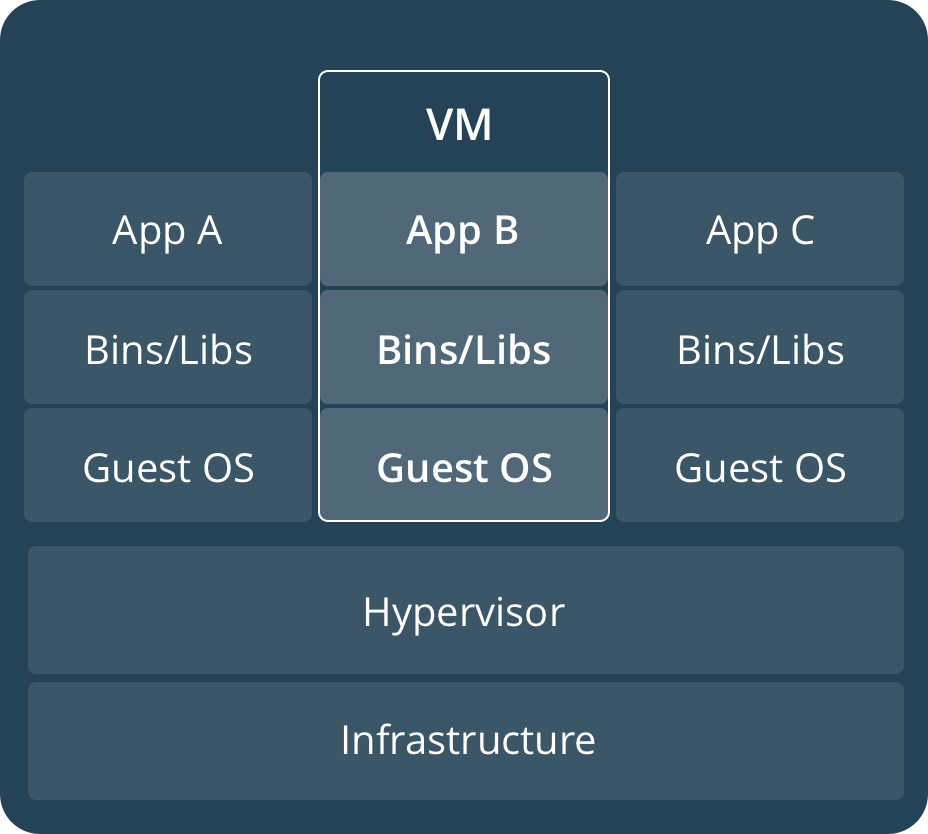
\includegraphics[scale=0.30]{vms.png}
            \caption{Máquinas virtuales sobre \textit{hypervisor}}
        \end{figure}

        \pagebreak


    \subsection{Plataformas de contenedores}
        Por otro lado existen también los \textbf{contenedores}, que el sitio de \docker{} los describe como ``paquete ejecutable liviano y autónomo de una pieza de software que incluye todo lo que necesita para correr: código, librería del sistema, configuraciones''. 
        
        Los contenedores son una abstracción en la capa de la aplicación que aislan el software que se desea ejecutar, armando un pequeño ambiente con las dependencias necesarias para que se ejecute solamente ese código. Esto facilita el trabajo de los desarrolladores, sabiendo que al trabajar y probar su producto en un contenedor, ese mismo contenedor podrá ser puesto en producción con la certeza de que funcionará, evitando incertidumbres que pueden generar intentar de ejecutar el software en distintos sistemas operativos o hardware.
        
        El sistema operativo anfitrión sobre el que corren los contenedores restringe el acceso del contenedor a los recursos físicos, por lo tanto un solo contenedor no podrá consumir todos los recursos del anfitrión. Como todos los contenedores comparten el kérnel del sistema operativo anfitrión, logran que su uso (también llamado \textit{virtualización basada en contenedores}) sea más eficiente que el uso de las máquinas virtuales (donde cada máquina virtual ejecutaba un sistema operativo entero)\\

        \begin{figure}
            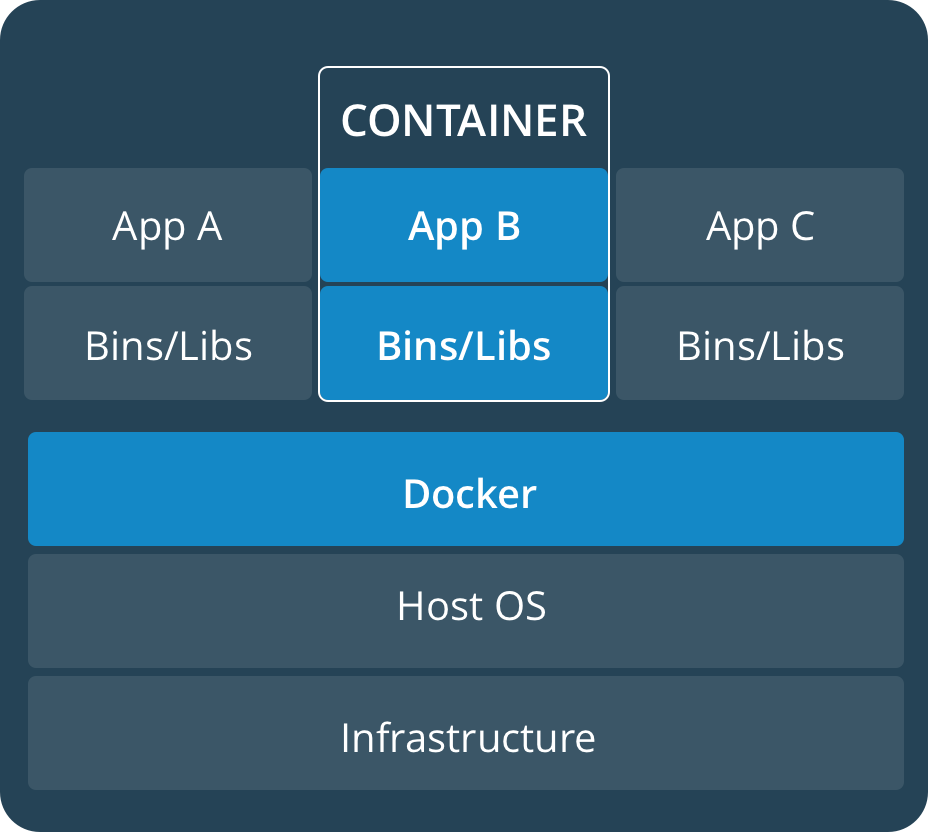
\includegraphics[scale=0.30]{containers.png}
            \caption{Contenedores corriendo sobre la plataforma \docker{}}
        \end{figure}

        \begin{quote}
            La diferencia clave entre los contenedores y las máquinas virtuales es que, mientras el \textit{hypervisor} abstrae un dispositivo entero, los contenedores solo abstraen el kérnel del sistema operativo. \cite{dockerdarnpopular}
        \end{quote}

        Al momento de momento de decidir si usar una máquina virtual o un contenedor para ejecutar una aplicación de forma aislada, no se debe perder de vista el \textbf{alcance} que se espera que tenga la aplicación.\cite{cloudinfrastructure}

        Al ser los contenedores mucho más livianos que las máquinas virtuales (no tienen que correr una instancia del sistema operativo, sólo la aplicación para la cual fueron diseñados), permiten elevar más el nivel de abstracción, logrando tener un contenedor altamente específico para correr una aplicación en particular.  Como práctica general, se mantiene el concepto de tener \textbf{un proceso por contenedor}.

        Por otro lado, las máquinas virtuales tienen un alcance mucho más amplio, permitiendo correr sistemas operativos enteros.  


    \clearpage
    \section{¿Qué es \docker{}?}
        
    \subsection{¿Qué \textbf{NO} es \docker{}?}
    \subsection{Arquitectura}


    hablar sobre lo que dice el informe, también hablar sobre registry (permite armar un repo local, y los clientes pueden descargar de ahí)

    \clearpage
    \section{Ventajas y desventajas}


    \clearpage
    \section{Ejemplo práctico}


    \clearpage
    \bibliographystyle{plainnat}
    \bibliography{tp_final}

\end{document}
